%%% CSE 4316 Individual Sprint Report - WORKED EXAMPLE (Mobile App + IoT)
\documentclass{article}
\usepackage{siunitx}\usepackage{graphicx}\usepackage{amsmath}
\setlength\parindent{0pt}
\usepackage[letterpaper, portrait, margin=1in]{geometry}
\title{Sprint 4 Report \\ CSE 4316}
\author{Charles Babbage}
\date{December 1st, 2026}
\begin{document}
\maketitle
\begin{center}
\begin{tabular}{l r}
Sprint start date: & November 17th, 2026 \\
Sprint end date: & December 1st, 2026 \\
Project title: & AquaGuard Smart Water-Leak Monitor \\
Team name: & Team Nimbus \\
Partners: 	& Alan Turing \\
			& Grace Hopper \\
			& John Von Neumann \\
        	& Ada Lovelace \\
Instructor: & Christopher D. McMurrough
\end{tabular}
\end{center}

\section{Sprint Goal}
Achieve reliable BLE pairing and a live sensor read from the device in the app on
both iOS and Android, ahead of the December milestone demo.

\section{Sprint Backlog}
Planned tasks (hours). \\
\begin{tabular}{| p{4in} | >{\centering\arraybackslash} p{1in} | >{\centering\arraybackslash} p{1in} |}
\hline
\textbf{Task description} & \textbf{Estimated work} & \textbf{Actual work} \\ \hline
Define GATT profile (services/characteristics) & 4.0 & 4.0 \\ \hline
Firmware: advertise + reading/battery characteristics & 6.0 & 7.0 \\ \hline
App: scan, pair/bond, subscribe (iOS) & 5.0 & 6.0 \\ \hline
App: same flow on Android + parity test & 5.0 & 5.5 \\ \hline
Bonded/encrypted link verification (SE-01) & 3.0 & 3.0 \\ \hline
Power sampling to seed the battery budget & 3.0 & 3.0 \\ \hline
\textbf{TOTAL} & \textbf{26.0}  & \textbf{28.5} \\ \hline
\end{tabular}

\pagebreak

\section{Individual Time Expenditures}
Tasks performed by the individual (hours). \\
\begin{tabular}{| p{4in} | >{\centering\arraybackslash} p{1in} | >{\centering\arraybackslash} p{1in} |}
\hline
\textbf{Task Description} & \textbf{Actual work} & \textbf{Percent complete} \\ \hline
Define GATT profile & 4.0 & 100\% \\ \hline
Firmware: advertise + characteristics & 7.0 & 100\% \\ \hline
Power sampling for battery budget & 3.0 & 80\% \\ \hline
\textbf{TOTAL} & \textbf{14.0}  & \textbf{-} \\ \hline
\end{tabular}

\section{Team Burndown Chart}
Ideal and actual daily team effort are shown below.
\begin{figure}[h]\begin{center}
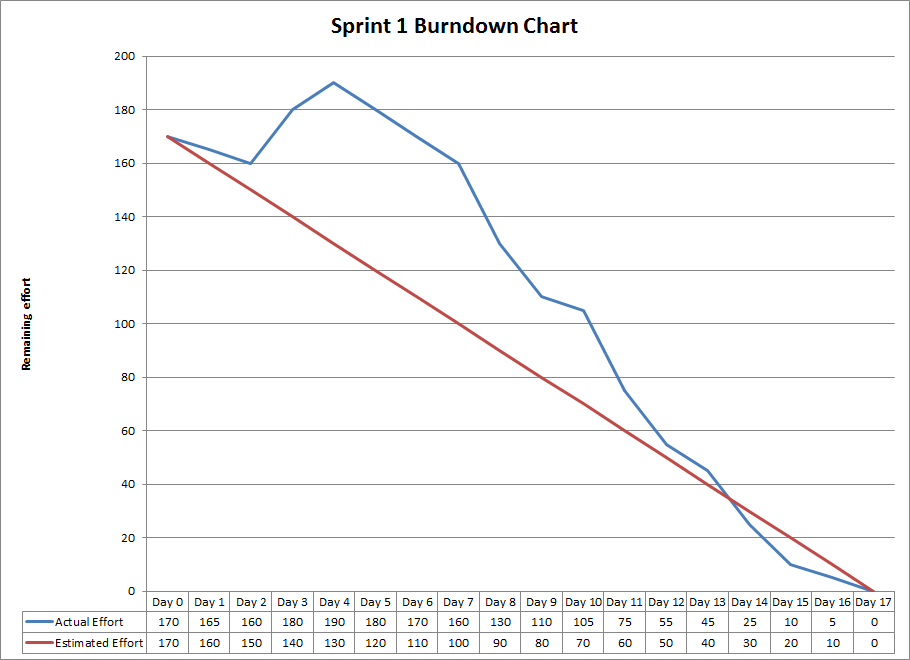
\includegraphics[width=1.0\textwidth]{images/burndown}
\end{center}\end{figure}

\pagebreak

\section{Individual Retrospective}
Actions to \textbf{start} doing (top 3)
\begin{itemize}
\item Test BLE background behavior on real iOS/Android devices each sprint, not at the end.
\item Record power measurements in a shared sheet to track the battery budget over time.
\item Freeze the GATT profile as a versioned interface doc before app work.
\end{itemize}
Actions to \textbf{stop} doing (top 3)
\begin{itemize}
\item Testing BLE only on the simulator/emulator.
\item Changing characteristic UUIDs without bumping the profile version.
\item Leaving the radio always-on during bench tests (skews battery numbers).
\end{itemize}
Actions to \textbf{continue} doing (top 3)
\begin{itemize}
\item Pairing with John on the BLE central/peripheral contract.
\item Keeping platform BLE differences isolated in one module (QA-01).
\item Short daily blocker syncs.
\end{itemize}

\section{Peer Review}
Candid individual assessment; not shared. Each item graded 1--5. \\
Evaluation items:
\begin{itemize}
\item \textbf{Participation} - present and contributing?
\item \textbf{Communication} - timely, effective updates?
\item \textbf{Work quality} - claimed tasks; met objectives; added value?
\item \textbf{Professionalism} - professional and collaborative?
\item \textbf{Overall} - overall value this period.
\end{itemize}
\begin{tabular}{| p{1.5in} | >{\centering\arraybackslash} p{1.in} | >{\centering\arraybackslash} p{1.1in} | >{\centering\arraybackslash} p{1.1in}| >{\centering\arraybackslash} p{0.5in}| >{\centering\arraybackslash} p{.5in} |}
\hline
\textbf{Team member name} & \textbf{Participation} & \textbf{Communication} & \textbf{Work quality} & \textbf{Professionalism} & \textbf{Overall} \\ \hline
Charles Babbage & 5 & 5 & 5 & 5 & 5\\ \hline
Alan Turing & 5 & 4 & 5 & 5 & 5\\ \hline
Grace Hopper & 4 & 5 & 4 & 5 & 4\\ \hline
John Von Neumann & 5 & 5 & 5 & 4 & 5\\ \hline
Ada Lovelace & 4 & 4 & 4 & 5 & 4\\ \hline
\end{tabular}
\end{document}
